\lecture[1]{Background}{lec:background}

\title{Background}
\subtitle{What you need to know}

\date{\today}

\begin{frame}
\maketitle
\end{frame}

\section{Classical Logic}

\begin{frame}{Overview of classical logic}
\begin{itemize}
    \item You should be familiar with \href{https://en.wikipedia.org/wiki/Boolean_algebra}{Boolean algebra} but we will review it here.
    \item The two constants
    \begin{itemize}
        \item \Zero{} or \False{}
        \item \One{} or \True{}
    \end{itemize}
    \item We will review functions over those values.
    \item Classical logic use \emph{bits} that are either \True{} or \False{}.
    \item Quantum logic uses \emph{qubits} that can be in a \emph{superposition} of \Zero{} and \One{}.
\end{itemize}
    
\end{frame}


\begin{frame}{Boolean functions of one input}
There are only two possible Boolean functions with just one input:
\begin{itemize}
    \item $f(x) = x$, the identify function
    \item $f(x) = \Not{x}$
\end{itemize}
The second function returns the \emph{complement} of the input value.  The operator is typically pronounced \emph{not}, and it is sometimes written $\neg x$.  In this class we will use the clearer \Not{x}.

The truth table for this function is simple:
\begin{center}
\begin{tabular}{c|c}
$x$  & \Not{x} \\
\hline
\Zero{} & \One{} \\
\One{} & \Zero{} \\
\end{tabular}
\end{center}
    
\end{frame}

\def\BTable#1#2#3#4#5{%
\begin{center}
\begin{tabular}{cc|c}
$x$ & $y$ & \ensuremath{#1} \\
\hline
\Zero{} & \Zero{} & \ensuremath{#2} \\
\Zero{} & \One{} & \ensuremath{#3} \\
\One{} & \Zero{} & \ensuremath{#4} \\
\One{} & \One{} & \ensuremath{#5} \\
\end{tabular}
\end{center}
}
\begin{frame}{Boolean functions of two inputs}
For two inputs $x$ and $y$, we generally have:
\BTable{f(x,y)}{f(0,0)}{f(0,1)}{f(1,0)}{f(1,1)}
With four possible results, each \Zero{} or \One{}, there are $2^4$ possible tables and so 16 possible boolean functions of two inputs.
\BigSkip{}
Some of those functions should be familiar.
\end{frame}

\begin{frame}{Conjunction and Disjunction}

\begin{columns}
\begin{column}{0.4\textwidth}
Conjunction

\BTable{x\wedge y}{0}{0}{0}{1}

The \emph{and} function is \True{} when both of its inputs are \True{}.

\only<2->{
We sometimes juxtapose inputs to imply conjunction:
\[x\wedge y = xy\]}
\end{column}
\begin{column}{0.4\textwidth}
Disjunction

\BTable{x\vee y}{0}{1}{1}{1}

The \emph{or} function is \True{} when either input is true, or both inputs are \True{}.

\only<2->{
We sometimes use $+$ as the operator for disjunction:
\[x\vee y = x + y \]}
\end{column}
\end{columns}
\end{frame}

\begin{frame}{Exclusive or}{This operation is prevalent in quantum computations.}

\BTable{\Xor{x}{y}}{0}{1}{1}{0}

Exclusive-or is what we usually mean in natural language when we say \emph{or}:
\MedSkip{}
\begin{quote}
    I am going to the gym or I am going to sleep.
\end{quote}
We mean we will do one or the other, but not both.
\end{frame}

\begin{frame}{Universality}{What operators are needed at a minimum?}
\begin{columns}
\begin{column}{0.5\textwidth}
Consider the function:
\end{column}
\begin{column}{0.5\textwidth}
\mbox{}\vskip -3em\mbox{}
\BTable{f(x,y)}{r_{00}}{r_{01}}{r_{10}}{r_{11}}
\end{column}
\end{columns}
\MedSkip{}
Any of the 16 possible functions can be written as:
\[
f(x,y) = \Not{x}\Not{y}\,r_{00} +\Not{x}y \,r_{01} + x\Not{y}\, r_{10} +xy \,r_{11} 
\]
For any $x,y$, exactly one of the above conjunctions involving $x$ and $y$ is true.  Thus, the above expression remains the same if $+$ is replaced by $\oplus$.  
\MedSkip{}
Based on the above, we see that universality is achieved using the three operators $\wedge$, $\vee$, $\neg$.
\end{frame}



\begin{frame}{Can we do better?}{Nand is a single, universal gate.}
\begin{columns}
\begin{column}{0.6\textwidth}
We define Nand as the not-of-and-of its two inputs:
\[
\mbox{Nand($x$,$y$)} = \Not{xy}
\]
\end{column}
\begin{column}{0.4\textwidth}
\BTable{\Nand{x,y}}{1}{1}{1}{0}
\end{column}
\end{columns}
\only<2->{
From this we can define:
\begin{eqnarray*}
\Not{x} & = & \Nand{x}{1} \\
\And{x}{y} & = & \Not{\Nand{x}{y}} \\
\only<3->{
\Or{x}{y} & = & \Nand{\Not{x}}{\Not{y}}}
\end{eqnarray*}
\MedSkip{}
\only<3>{
This follows from one of \href{https://en.wikipedia.org/wiki/De_Morgan\%27s_laws}{De~Morgan's laws}:
\[
\Not{uw} = \Or{\Not{u}}{\Not{w}}
\]
}
\only<4->{
We thus achieve universality with a single gate.
}
}
\end{frame}

\section{Complex arithmetic}

\begin{frame}{Overview of complex arithmetic}
\begin{itemize}
    \item Complex arithmetic is especially convenient for quantum computing.
    \item We will use both forms:
    \begin{itemize}
        \item \href{https://en.wikipedia.org/wiki/Cartesian_coordinate_system}{Cartesian coordinates}
        \item \href{https://en.wikipedia.org/wiki/Polar_coordinate_system}{Polar coordinates}
    \end{itemize}
    \item Complex values allow us to express the magnitude of a wave as well as its phase.  This is helpful for understanding interference.
    \item We could defer using complex arithmetic in this course, but it is wise to embrace it from the start.
\end{itemize}
\end{frame}

\begin{frame}{Complex Numbers}{Cartesian coordinates}
  
  \TwoColumns
    \adjustbox{valign=t}{%
    \begin{tikzpicture}[scale=0.7]
  \only<1->{
  \draw[<->] (-2, 0) -- (2.5, 0) node[right] {real};
  
  \draw[->] (0, 0) -- (1, 0) node[below] {$a$} ;

  }
  
  \visible<2->{
  \draw[<->] (0, -2) -- (0, 2.5) node[above] {imaginary};
  
  \draw[->] (0, 0) -- (0, 2) node[left] {$b$} ;
  
  }
  \only<3->{
  \draw[->] (0, 0) -- (1, 2) ;
  \draw[fill=black]
        (1.05,2.05) circle (2pt) node[above right] {$z=a+bi$} ;
  }
  \only<4->{
  \draw[->] (0, 0) -- (1, -2) ;
  \draw[fill=black]
        (1.05,-2.05) circle (2pt) node[below right] {$\Conj{z}=a-bi$} ;
  }
\end{tikzpicture}}
}
\only<4->{\BigSkip{}The \emph{magnitude} of $z$ is given by $\Mag{z} =  \sqrt{a^{2}+b^{2}}$.}\only<5->{  We thus obtain:
\[
 \Mag{z}^{2}  =  a^{2}+b^{2} = z\Conj{z} = \Conj{z}z
\]
}
\end{frame}

\begin{frame}{The complex unit circle}{All points on the circle have unit length.}
\end{frame}


\begin{frame}{From Cartesian to polar coordinates}
    
\end{frame}

\section{Linear algebra}

\begin{frame}{Overview of linear algebra}{Quantum systems are linear!}
\begin{itemize}
    \item While much of our world behaves nonlinearly, quantum systems can surprisingly be captured using linear algebra.
    \item Vectors and matrices can represent states and gates.  
    \begin{itemize}
        \item The state of a quantum system is most often described as a column vector, called a \href{https://en.wikipedia.org/wiki/Bra-ket_notation}{ket}.
         \item The effect of a quantum gate can be described as a square matrix, which maps in input ket to an output ket.
    \end{itemize}
    \item This is convenient but not efficient in the number of quantum bits.
    \item The composition of states and gates is computed using \href{https://en.wikipedia.org/wiki/Tensor}{tensor arithmetic}.
\end{itemize}
    
\end{frame}

\begin{frame}{Bra-ket notation}{Describing quantum states}
Quantum computing borrows notation from physics in using \href{https://en.wikipedia.org/wiki/Paul_Dirac}{Paul Dirac}'s \href{https://en.wikipedia.org/wiki/Bra-ket_notation}{bra-ket} notation.
\TwoColumns{%
\begin{itemize}
\item<1-> We typically represent a quantum state using a column vector.


\item<2-> Dirac calls such a vector a \emph{ket}, using this syntax that looks strange, but will soon become useful.

\end{itemize}
}{
\[
\only<2->{\ket{\psi} = }
\begin{pmatrix}
0.5\\ i \\ 5+3i \\ \sqrt{2}

\end{pmatrix}
\]
    
}
\only<1-2>{
\Remark{%
We will soon define and study the meaning of a vector's components, but for now it's just math.}
}
\only<3->{\BigSkip{} The \emph{bra} of a ket is its conjugate transpose, and \VV{}.
\[
\bra{\psi} =
\begin{pmatrix}
0.5 & -i & 5-3i &  \sqrt{2}
\end{pmatrix}
\]
}
\end{frame}

\begin{frame}{Inner Products}
The complete bra-ket of a state is the inner product of its bra with its ket, which computes the magnitude of the state, squared:
\begin{eqnarray*}
\braket{\psi}{\psi} & = &
\begin{pmatrix}
0.5 & -i & 5-3i &  \sqrt{2}
\end{pmatrix}
\times\begin{pmatrix}
0.5\\ i \\ 5+3i \\ \sqrt{2}
\end{pmatrix}
\\
 & = & 0.5^{2} + -i^{2} + 25-9i^{2} + 2 
\end{eqnarray*}
    
\end{frame}


